\subsection{Quest Generation}

\begin{figure*}[t]
    \centering
    \captionsetup[subfigure]{width=0.9\textwidth}
    \begin{subfigure}[t]{1\textwidth}
        \centering
        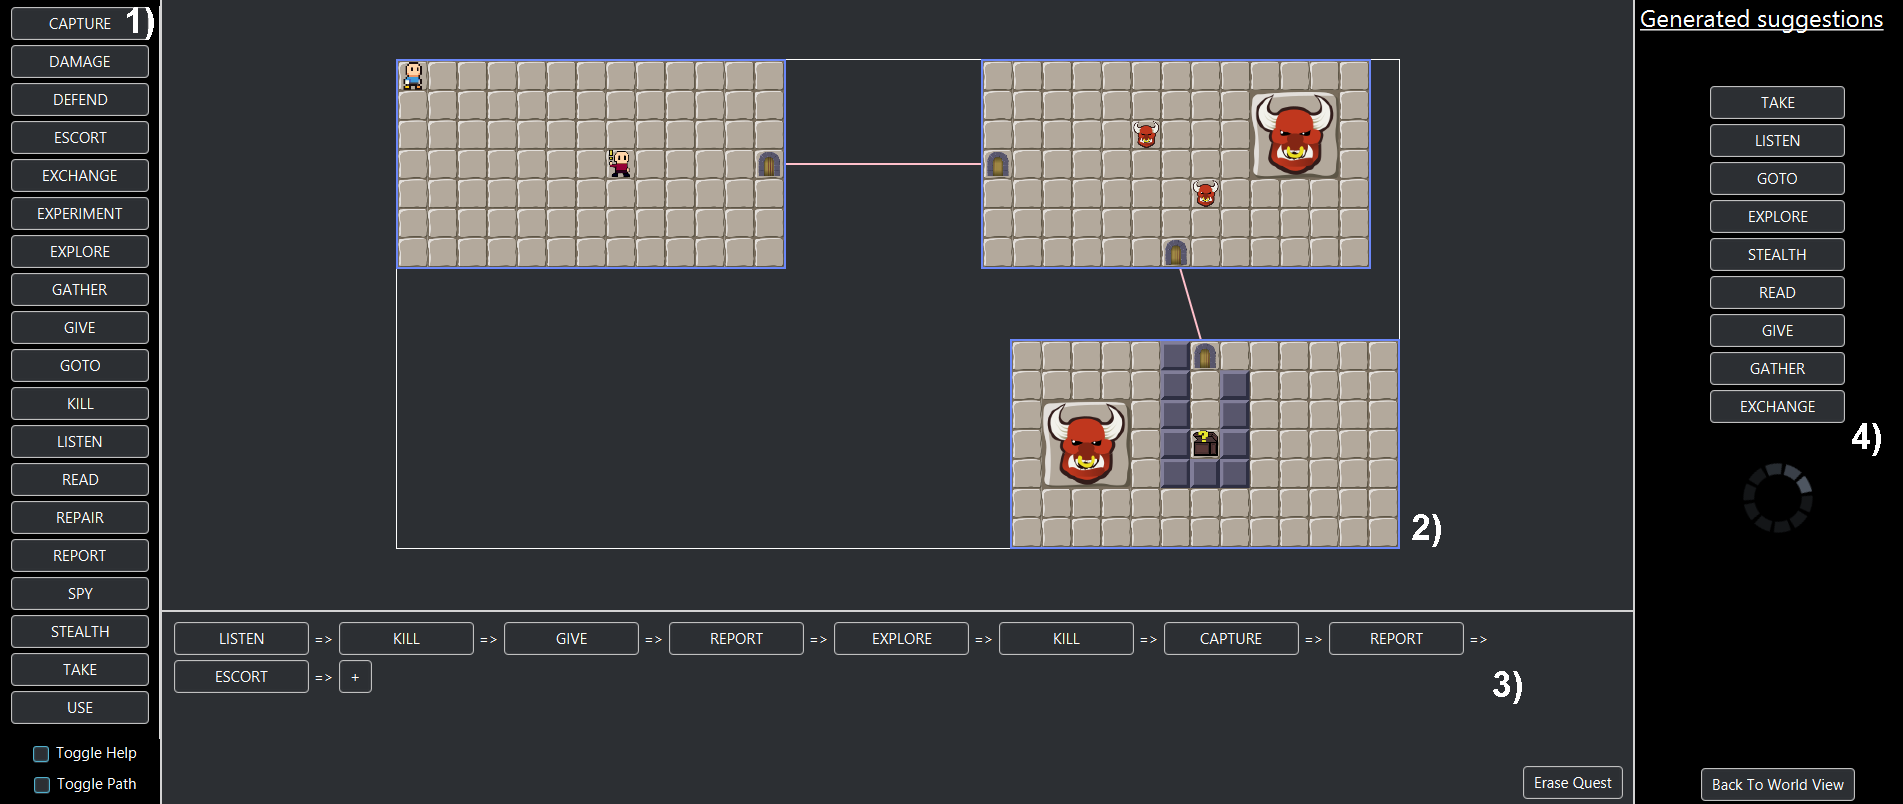
\includegraphics[width=.9\textwidth]{included-papers-tex/paper-8/figures/main.png}
        \caption{Overview of the GUI used for the design of quests in EDD. 1) The possible quest actions, 2) the dungeon created thus far by the designer, 3) the quest sequence, and 4) the suggestions from the grammar.}
        \label{figs:GUI:overview}
    \end{subfigure} \hfill% \
     
    \begin{subfigure}[t]{0.48\textwidth}
        \centering
         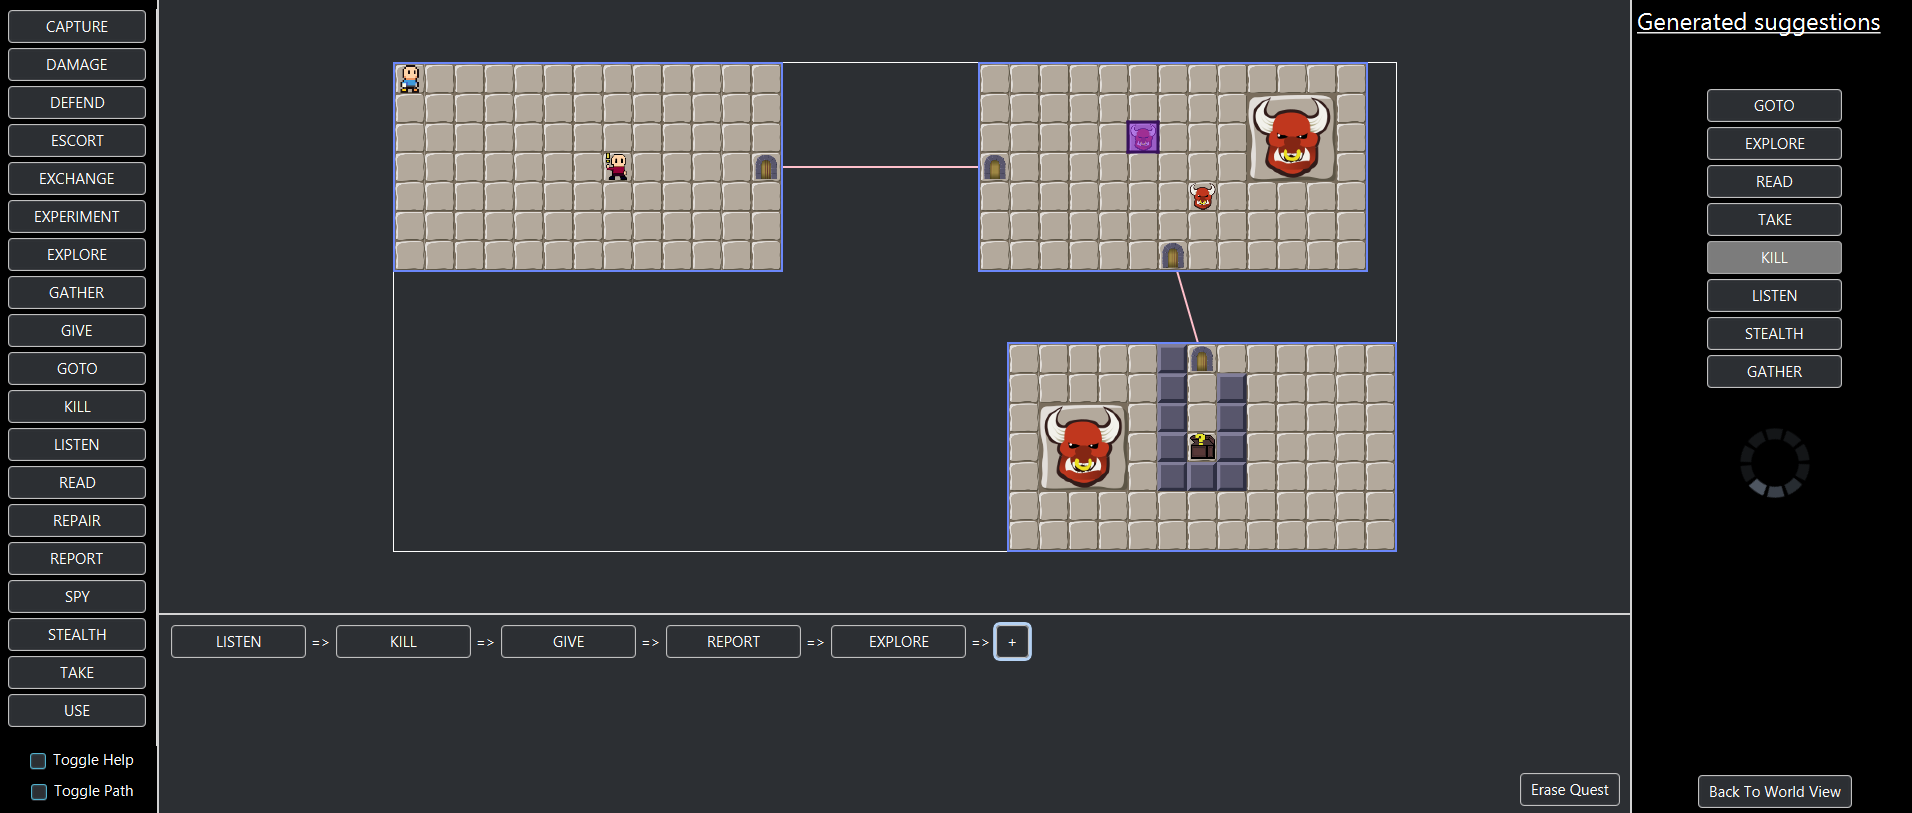
\includegraphics[width=1\textwidth]{included-papers-tex/paper-8/figures/main-sug.png}
        \caption{An example quest sequence and the user attempting to select a suggested quest action}
        \label{figs:GUI:suggestions}
    \end{subfigure}
    \begin{subfigure}[t]{0.48\textwidth}
        \centering
        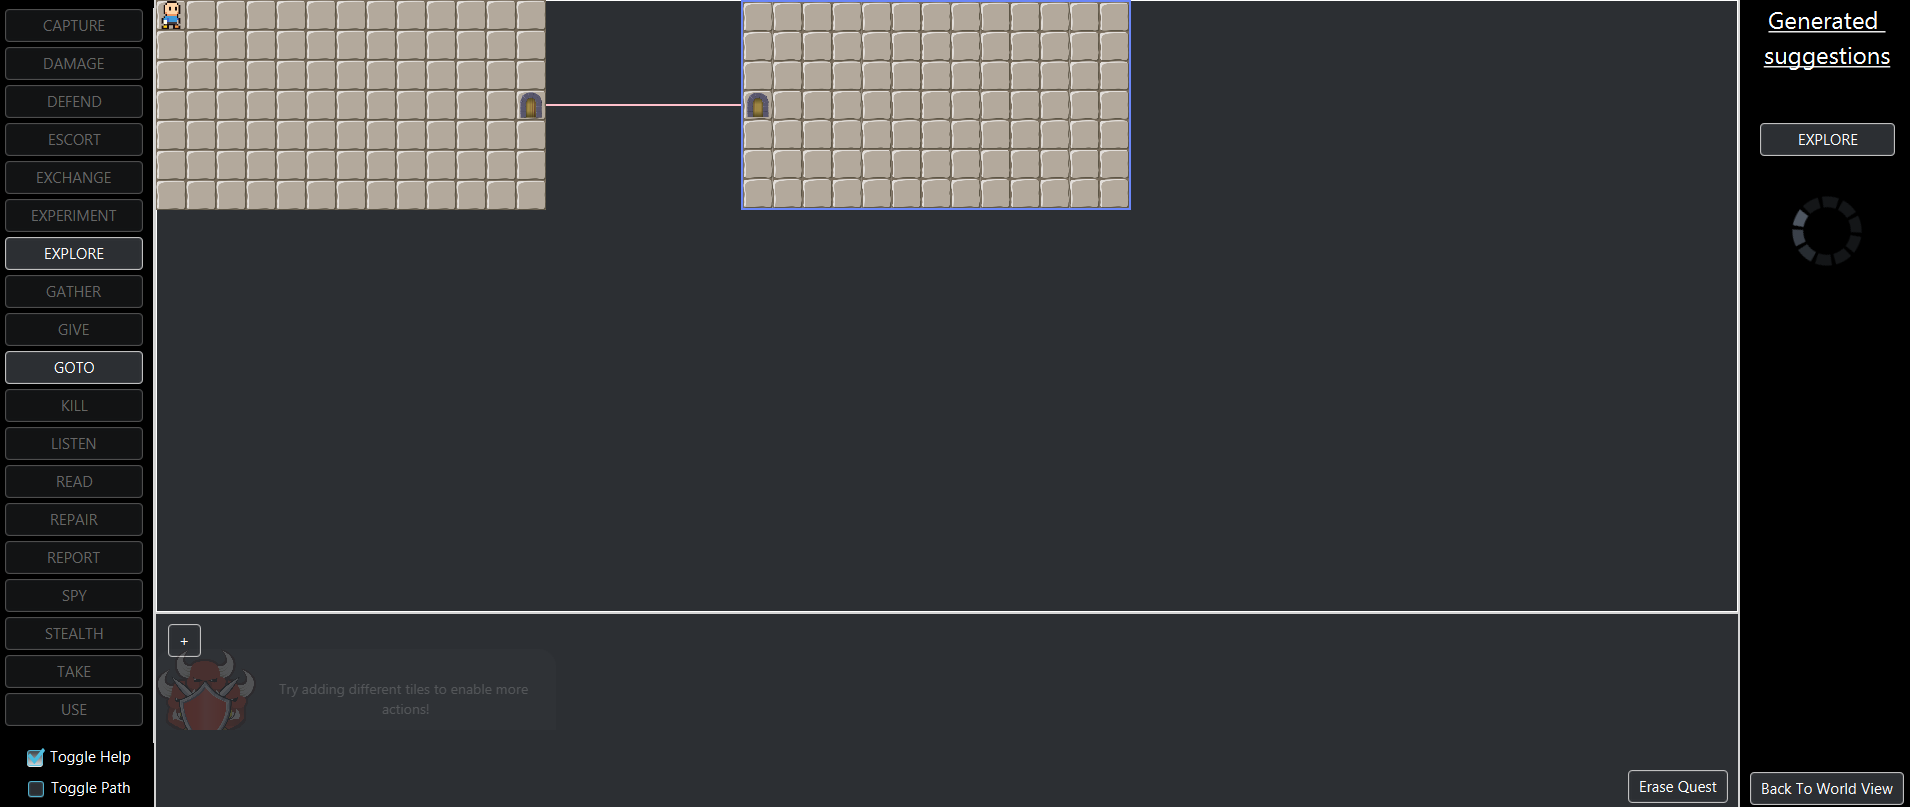
\includegraphics[width=1\textwidth]{included-papers-tex/paper-8/figures/main-available-quest.png}
        \caption{Example of two empty and connected rooms, where most prerequisites for quest actions are not met.}
        \label{figs:GUI:avQuest}
    \end{subfigure} \hfill%
     \begin{subfigure}[t]{0.48\textwidth}
        \centering
        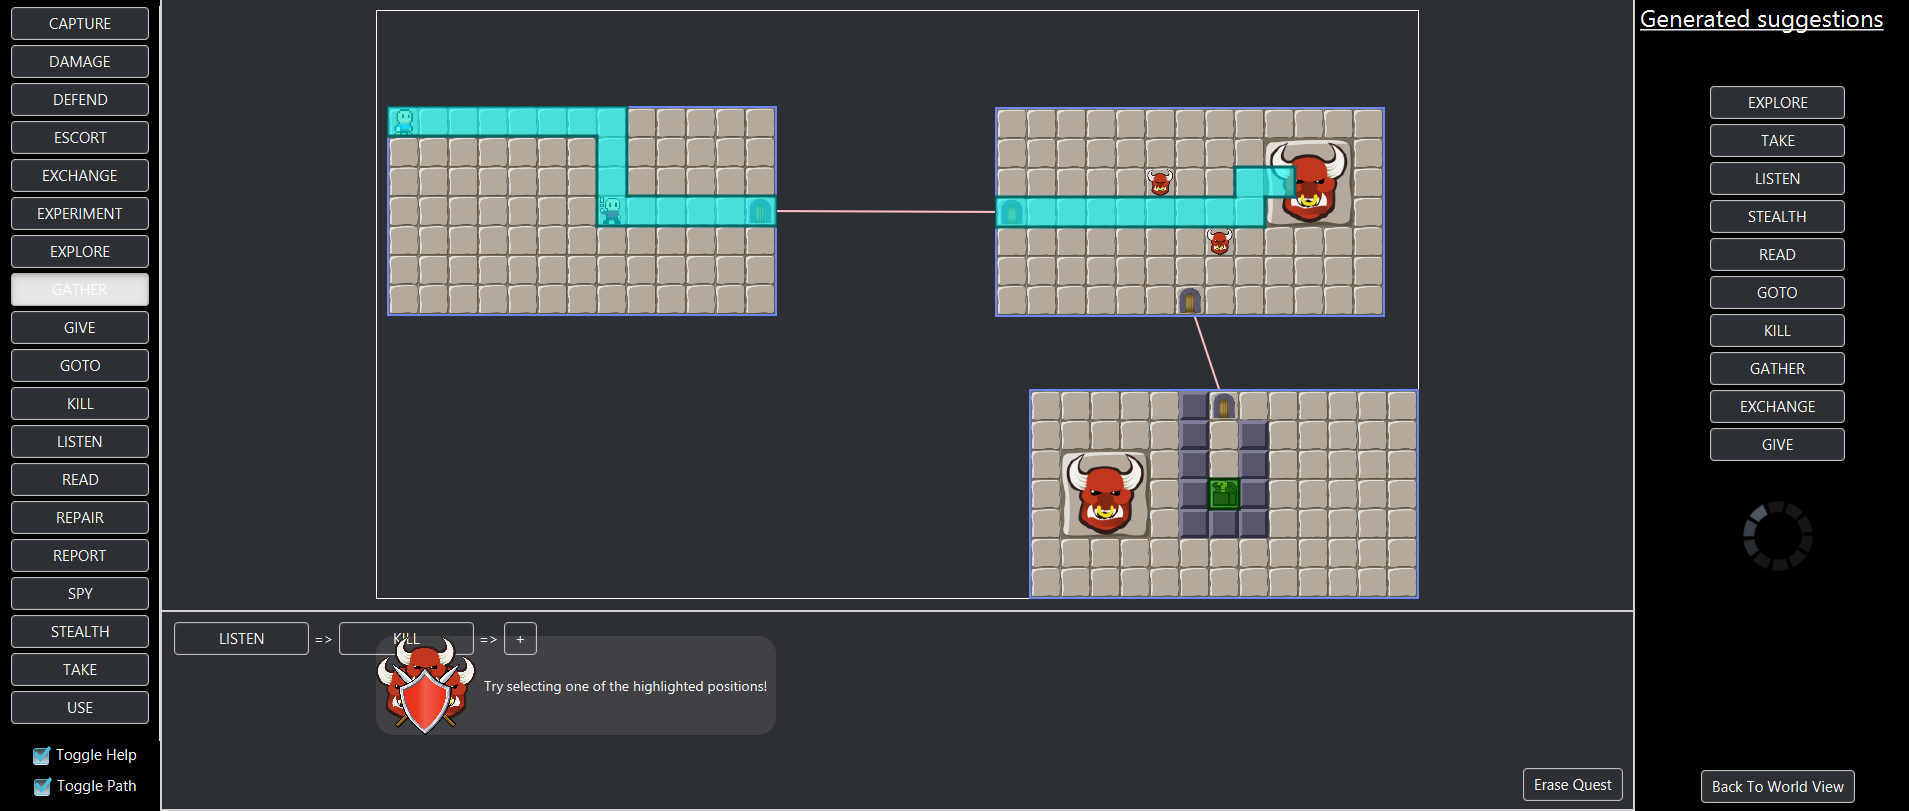
\includegraphics[width=.99\textwidth]{included-papers-tex/paper-8/figures/main-help.png}
        \caption{Example of the provided help for designers. A pop-up informs them of events, and in cyan, the A* path.}
        \label{figs:GUI:help}
    \end{subfigure}%
     \begin{subfigure}[t]{0.48\textwidth}
        \centering
        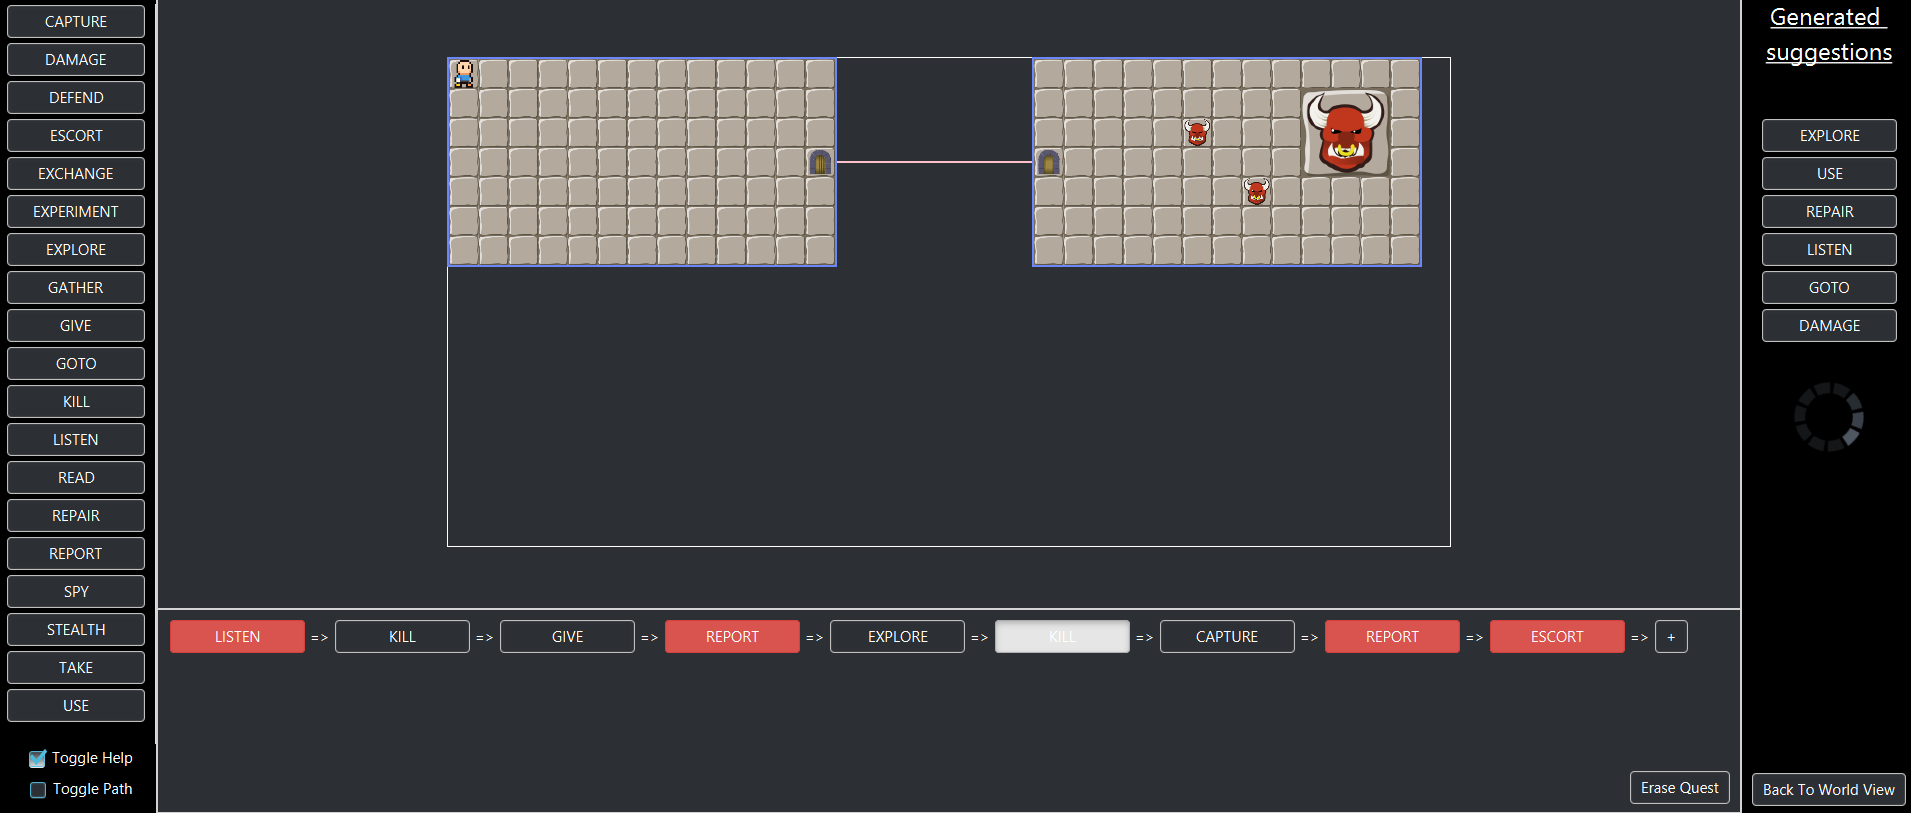
\includegraphics[width=.99\textwidth]{included-papers-tex/paper-8/figures/main-errorQ.png}
        \caption{Error in the quest sequence since the designer erased a room containing quest action tiles.}
        \label{figs:GUI:error}
    \end{subfigure} \hfill%
    \caption{Visualization of the GUI used for creating quest sequences and different states}
    \label{figs:GUI}
\end{figure*}

Questgram is a quest generation tool that lets the designer compose one long sequence of quest actions to create an overarching objective for the dungeon they are creating. These quest actions are based on the quest analysis and classification and produced grammar by Doran and Parberry~\citepeighth{p8Doran2011-questsMMORPGs}. Questgram builds on top of EDD extending its level design and generation capabilities with a mixed-initiative quest editor and takes advantage of its mixed-initiative perspective and the level design system.


% , where a set of nine NPC motivations were extracted, and formed as a production rules for a grammar. Our system is implemented on top of EDD, extending its level design and generation capabilities with a mixed-initiative quest editor. 

%Therefore, EDD needed to be extended with some key elements such as a new quest editor view and new tiles such as and NPC (i.e., quest giver)

% Following Yu et al. formal definition, each quest action would be a task $t$, which is represented by a 4-tuple $\langle C, M, I, R_{t} \rangle$, where $C$ are the game elements created by the designer linked to a quest action as described in table~\ref{table:prereq} and the grammar itself. $M$ is the level editor in EDD. $I$ is partially disregarded as the quest are not presented to players, but integrated as a sequence list shown in figure~\ref{figs:GUI:overview}. Lastly, as the system creates an overarching quest rather than $R_{t}$ is implicitly incorporated when set

% Following Yu et al. formal definition, a quest in Questgram is a long sequence of quest actions or tasks that must be fulfilled sequentially. 

%Perhaps some formal definition?

EDD was extended with some key elements such as a new quest editor view depicted in figure~\ref{figs:GUI:overview}, and two new generic tiles; an NPC acting as quest giver and target, and a quest item, which is the subject of many quests. These two new tiles were kept as generic as possible for future systems to have the responsibility of handling what type of NPC and object should replace those, similarly as with the other tiles in EDD such as the generic enemy, boss, and treasure. These tiles, together with the pre-existing enemy and boss tiles, have been intertwined with the actions, resulting in the "unlocking" mechanism of different quests, which can be observed in table~\ref{table:prereq}. It must be noted that while Questgram integrates and utilizes the different features and tiles of EDD's level generation facet, there is no integration of the new tiles and quests with EDD's evolutionary algorithm IC MAP-Elites~\citepeighth{p8Alvarez2020-ICMAPE}. This is left for future work.

While games can be either linear, semi-open, or open, with branching narratives and the design structured by the types of quests featured in a game~\citepeighth{p8aarseth2005hunt}, with concepts such as kernels and satelites~\citepeighth{p8Aarseth2012-Narrativetheory}; our approach only allows for the creation of a single overarching quest.

% our system forces the game to be linear. 

% Furthermore, our approach only let designers create one single overarching quest, which can be seen as a set of subquests.

% One limitation of our system is that it only allows for a single overarching quest, which can be seen as a set of quests, 

% While games can be either linear, semi-open, or open, and the design is structured by the types of quests featured in a game~\citepeighth{p8aarseth2005hunt}, with concepts such as kernels and satelites~\citepeighth{p8Aarseth2012-Narrativetheory}; our system forces the game to be linear. 

\subsubsection{Quest Actions}

% Please add the following required packages to your document preamble:
% \usepackage{graphicx}
\begin{table*}[]
\caption{displaying the actions together with Doran and  Parberry's~\cite{Doran2011-questsMMORPGs} prerequisites and how the actions and the previously mentioned prerequisites have been implemented in EDD. This indirectly explains the “unlocking” - describing what tiles that must be placed for an action to be available. Note that “Goto” \& “Explore” do not have any special tile prerequisites besides available floor. }
\label{table:prereq}
\resizebox{\textwidth}{!}{%
\begin{tabular}{lll}
\hline
Action   & Prerequisites in~\cite{Doran2011-questsMMORPGs} & Prerequisites in EDD \\ \hline
Capture    & “Somebody is there”                          & A NPC or boss/enemy must be placed.                        \\
Damage     & “Somebody or something is there”             & An item or NPC must be placed.                             \\
Defend     & “Somebody or something is there”             & An item or NPC must be placed.                             \\
Escort     & “Somebody is there”                          & A NPC must be placed.                                      \\
Exchange & “Somebody is there, they and you have something”          & A NPC and an item must be placed (requires two positions). \\
Experiment & “Something is there”                         & An item must be placed.                                    \\
Explore    & “none”                                       & An available floor tile.                                   \\
Gather     & “Something is there.”                        & An item must be  placed.                                   \\
Give       & “Somebody is there, you have something.“     & A NPC and an item must be placed (requires two positions). \\
Goto       & “You know where to go and how to get there.“ & An available floor tile.                                   \\
Kill       & “Somebody is there.“                         & A boss/enemy must be placed.                               \\
Listen     & “Somebody is there.“                         & A NPC must be placed.                                      \\
Read       & “Somebody is there.“                         & A NPC must be placed.                                      \\
Repair     & “Somebody is there.“                         & A NPC must be placed.                                      \\
Report     & “Somebody is there.“                         & A NPC must be placed.                                      \\
Spy        & “Somebody or something is there.“            & A NPC or boss/enemy must be placed.                        \\
Stealth    & “Somebody is there.“                         & A NPC or boss/enemy must be placed.                        \\
Take       & “Somebody is there, they have something.“    & A NPC and an item must be placed (requires two positions). \\
Use        & “There is something there.“                  & An item must be placed.                                    \\ \hline
\end{tabular}%
}
\end{table*}

\begin{table}[]
\caption{displaying the grammatical rules. The columns marked with asterisks are identified as “motivations” by Doran and Parberry~\cite{Doran2011-questsMMORPGs}, but are used as a starting point for the quests. The “\textless \textgreater{}” indicates the next production rule to be taken, and actions without “\textless \textgreater{}” is  the terminating action.}
\label{tab:productionRules}
\resizebox{\textwidth}{!}{
\begin{tabular}{ll}
\hline
Production   rules &
  Actions \\ \hline
knowledge* &
  {[}"\textless{}get\textgreater{}","\textless{}go\_to\textgreater{}","give"{]},   {[}"\textless{}spy\textgreater{}"{]}, \\
  &
  {[}"\textless{}go\_to\textgreater{}","listen","\textless{}go\_to\textgreater{}","report"{]}, \\
 &
  {[}"\textless{}get\textgreater{}","\textless{}go\_to\textgreater{}","use","\textless{}go\_to\textgreater{}","give"{]} \\
comfort* &
  {[}"\textless{}get\textgreater{}","\textless{}go\_to\textgreater{}","give"{]},\\
  &
  {[}"\textless{}go\_to\textgreater{}","damage","\textless{}go\_to\textgreater{}","report"{]} \\
reputation* &
  {[}"\textless{}get\textgreater{}","\textless{}go\_to\textgreater{}","give"{]},   \\
 &
 {[}"\textless{}go\_to\textgreater{}","\textless{}kill\textgreater{}","\textless{}go\_to\textgreater{}","report"{]}, \\
 &
  {[}"\textless{}go\_to\textgreater{}","\textless{}go\_to\textgreater{}","report"{]} \\
serenity* &
  {[}"\textless{}go\_to\textgreater{}","damage"{]},   \\
 &
 {[}"\textless{}get\textgreater{}","\textless{}go\_to\textgreater{}","use","\textless{}go\_to\textgreater{}","give"{]}, \\
 &
  {[}"\textless{}get\textgreater{}","\textless{}go\_to\textgreater{}","use","capture","\textless{}go\_to\textgreater{}","give"{]}, \\
 &
  {[}"\textless{}go\_to\textgreater{}","listen","\textless{}go\_to\textgreater{}","report"{]},   \\
 &
 {[}"\textless{}go\_to\textgreater{}","take","\textless{}go\_to\textgreater{}","give"{]}, \\
 &
  {[}"\textless{}get\textgreater{}","\textless{}go\_to\textgreater{}","give"{]},   \\
 &
 {[}"\textless{}go\_to\textgreater{}","damage","escort","\textless{}go\_to\textgreater{}","report"{]} \\
protection* &
  {[}"\textless{}go\_to\textgreater{}","damage","\textless{}go\_to\textgreater{}","report"{]},   \\
 &
 {[}"\textless{}get\textgreater{}","\textless{}go\_to\textgreater{}","use"{]}, \\
 &
  {[}"\textless{}go\_to\textgreater{}","repair"{]},   {[}"\textless{}get\textgreater{}","\textless{}go\_to\textgreater{}","use"{]},   \\
 &
 {[}"\textless{}go\_to\textgreater{}","damage"{]}, {[}"\textless{}go\_to\textgreater{}","repair"{]}, \\
 &
     {[}"\textless{}go\_to\textgreater{}","defend"{]} \\
conquest* &
  {[}"\textless{}go\_to\textgreater{}","damage"{]},   {[}"\textless{}go\_to\textgreater{}","\textless{}steal\textgreater{}","\textless{}go\_to\textgreater{}","give"{]} \\
wealth* &
  {[}"\textless{}go\_to\textgreater{}","\textless{}get\textgreater{}"{]},   {[}"\textless{}go\_to\textgreater{}","\textless{}steal\textgreater{}"{]}, {[}"repair"{]} \\
ability* &
  {[}"repair","use"{]},   {[}"\textless{}get\textgreater{}","use"{]}, {[}"use"{]},   {[}"damage"{]}, \\
 &
  {[}"\textless{}get\textgreater{}","experiment"{]} \\
equipment* &
  {[}"repair"{]},   {[}"\textless{}get\textgreater{}","\textless{}go\_to\textgreater{}","give"{]},   {[}"\textless{}steal\textgreater{}"{]},\\
 &
  {[}"\textless{}go\_to\textgreater{}","exchange"{]} \\
subquest* &
  {[}"\textless{}go\_to\textgreater{}"{]},   {[}"\textless{}go\_to\textgreater{}","\textless{}QUEST\textgreater{}","go\_to"{]} \\
go\_to &
  {[}"explore"{]},   {[}"\textless{}learn\textgreater{}","go\_to"{]} \\
learn &
  {[}"\textless{}go\_to\textgreater{}","\textless{}subquest\textgreater{}","listen"{]},   \\
 &
 {[}"\textless{}go\_to\textgreater{}","\textless{}get\textgreater{}","read"{]}, \\
 &
  {[}"\textless{}get\textgreater{}","\textless{}subquest\textgreater{}","give","listen"{]} \\
get &
  {[}"\textless{}steal\textgreater{}"{]},   {[}"\textless{}go\_to\textgreater{}","gather"{]}, \\
 &
  {[}"\textless{}go\_to\textgreater{}","\textless{}get\textgreater{}","\textless{}go\_to\textgreater{}","\textless{}subquest\textgreater{}","exchange"{]} \\
steal &
  {[}"\textless{}go\_to\textgreater{}","stealth","take"{]},   {[}"\textless{}go\_to\textgreater{}","\textless{}kill\textgreater{}","take"{]} \\
spy &
  {[}"\textless{}go\_to\textgreater{}","spy","\textless{}go\_to\textgreater{}","report"{]} \\
capture &
  {[}"\textless{}get\textgreater{}","\textless{}go\_to\textgreater{}","capture"{]} \\
kill &
  {[}"\textless{}go\_to\textgreater{}","kill"{]} \\ \hline
\end{tabular}
}
\end{table}

Doran and Parberry identified 19 different actions to be used as quest actions~\citepeighth{p8Doran2011-questsMMORPGs}, which we implemented and where each has its contextual prerequisites to be able to add them. In some cases, we have decided regarding if the actor represented in the action is friendly, e.g., NPC, or hostile, based on the tool's nature and the levels created. These actions are available for both the grammar and the designer to create as many steps as wanted in the overarching quest. The actions, their original prerequisite, and the domain-specific prerequisite are depicted in table~\ref{table:prereq}. 

These actions can be added one after each other in any order by the designers allowing for combinations and quests outside of the possible grammar seen in table~\ref{tab:productionRules}. Besides manual creation, the designer can instead pick a suggested action from the generated actions from the right panel, which offers the next action to be added to the quest. After deciding these options, the user will need to press the "+" button on the bottom panel, which will add the action to the quest sequence.


% Based on Doran and Parberry's work, we implemented 19 different actions to be used as quest actions~\citepeighth{p8Doran2011-questsMMORPGs},. In some cases, we have made the decision regarding if the actor represented in the action is friendly e.g., NPC or hostile e.g., enemy given the nature of the tool and the levels created. These actions are available for both the grammar and the designer to create as many steps as wanted in the overarching quest.  The actions are depicted in table~\ref{tab:prerequisites}, which also shows 

% These actions can be added one after the other one in any order by the designers allowing for combinations and quests outside of the possible grammar seen in table~\ref{tab:grammar}

% In order for designer to add some actions, they require some prerequisites 

% 19 different actions have been added to the quest implementation. These are based on Parberry and Dorans research [8]. However in some cases, we have made the decision regarding if the actor represented in the action is friendly (NPC) or hostile (enemy), this will be evaluated in the user feedback.  The actions have different prerequisites (table 1). With the actions “unlocking” through the user placing the necessary tiles. The user has the option to select what type of action and then what position on the map the action will take place. This is done by selecting a specific floor tile, marking that position on the map. However, Exchange, Give, and Take requires two positions due to its two subject nature (an actor + an item). 

% Besides manual placement, the user has the option to instead pick a suggested action from the generated actions from the right panel. After deciding these options, the user will need to press the “+” button on the bottom panel, this will add the action to the quest sequence

\subsubsection{Quest Grammar}

The system employs a generative grammar, specifically Lindenmayer Systems (L-Systems)~\citepeighth{p8Lindenmayer1996-LSystems} to generate the different set of quests using the production rules depicted in table~\ref{tab:productionRules}. The production rules are divided into two categories: 1) motivations for NPCs to start a quest such as~\emph{knowledge} where the focus would be to create quests with more passive actions or~\emph{reputation} where the focus would be to kill some enemy to gain reputation with some NPC. 2) Non-motivation rules related to the development of quests (i.e., non-terminal symbols) such as "go\_to" or "get". In table~\ref{tab:productionRules} non-terminal symbols are represented with "<" and ">", and terminal symbols simply list the action.

% The system can generate complete quests on its own by using one of the NPC Motivations as axiom, but when used in a mixed-initiative fashion with the designer manually creating the quests, the system uses the current active quest sequence created by the designer. The system then proposes a set of valid quest items to the designer to continue the quest or replace a current action. 

The system can be used for generating complete quests on its own, which select one of the NPC motivations as an axiom or with the designer in a mixed-initiative approach. As a mixed-initiative approach, the designer can manually create a quest sequence while the system uses the current quest sequence to suggest a set of valid quest items to the designer to continue the quest or replace a current action. Given that the production rules are invariable, there can be situations where the system cannot generate quests based on the quest sequence. This would result in the designer receiving feedback that the quest is not compatible with the grammar itself, giving the designer suggestions on how to continue and overcome this limitation.

Quest actions are suggested to continue the current sequence and append a new action at the end, or they can be used to replace an action in any position of the current sequence. For both, the system continuously produce quests using the grammar and filters out those that do not match the designer's sequence up to the position where they wish to change a quest action. In this way, the designer can choose suggestions for either continuing and finishing the quest or replacing existing parts for other valid actions.

% In the latter, the sequence up to the position where the designer wishes to change a quest action 

% change an action is used as axiom of the quest generator. In this way, the designer is given the option to choose suggestions for either continuing and finishing the quest or replace existing parts for other valid actions.

% Through this, the quest sequence might become unusable for the grammar to produce new suggestions, given that a sequence might not exist, but since the . We acknowledge this as a limitation of the system

\subsubsection{Workflow}

The GUI for the quest generation system of EDD follows the same concept and design as the room editor for consistency. Placeable quest actions are at the left pane, and generated suggestions with the grammar are at the right pane. The whole dungeon can be seen on the center top pane, and at the center bottom, the designer can compose the quest. These parts can be explicitly seen in figure~\ref{figs:GUI:overview}.

The designer cannot add any quest action, which prerequisite has not been fulfilled yet as described in table~\ref{table:prereq} and exemplified in figure~\ref{figs:GUI:avQuest}. Quest actions need to be linked to some actual tile representation in the dungeon. For instance, a "KILL" action requires selecting an enemy, while the "GO TO" requires any floor tile. Therefore, once the designer adds a new quest action, they must choose which tile is linked to this, presented to the designer in green. Similarly, when a quest action is suggested, the system randomly picks an available tile shown in purple to the designer as shown in figure~\ref{figs:GUI:suggestions}.

Moreover, the sequence panel is displayed in fig. 7.4. The panel displays the actions the user has selected. To add a sequence to the list, the user needs to manually select an action and its desired position or select a suggested action. Both of these options require the user to press the "+" button manually. Similarly, each quest action in the sequence is clickable and interchangeable. If a quest action in the sequence is selected, the designer can exchange it by selecting the quest action desired from the action panel or from the newly suggested actions, or remove it.

Finally, the designer can toggle two different types of assistance. The first focuses on informing the designer of changes in the sequence due to a manually placed or automatically generated, and informs the designer of the tile that needs to be selected. The second assistance shows A* paths between the target tile of a selected quest action and the next target tile. Both assistance is depicted in figure~\ref{figs:GUI:help}.

% The user interface for quest-tool implementation follows the room-view’s design, and consists of four panels; the left-hand toolbar, the right-hand generated suggestions, the central map-view, and the bottom quest-panel (fig. 7).

% 4.3.2.1 Action tiles

% Since EDDs world map is reused in the quest tools, all of EDDs pre-existing visual elements remain the same in the quest view. An action takes up 1x1 square which is the general size of tile elements in EDD, however a boss requires 4x4 tiles, though this is still treated as 1x1 entity, and thus an 1x1 tile of the 4x4 is required to be selected. Once an action is placed on the room manually, the available tiles where the action can be placed will be displayed in green (fig. 2). When the user selects a suggestion from the generator, the available tiles will instead be displayed in purple (fig. 3). 
  
% Figure 2 displaying an user manually selecting the “listen” action, therefore the NPC will be highlighted in green to display its availability.

% Figure 3 displaying a user selecting a generated suggestion, “give”, the generator automatically selects the required tiles and highlights them in purple. 

% 4.3.2.2 Action panel

% The action panel is displayed in fig. 7.1. The panel consists of buttons for each respective action (19 actions). The tile placed in the room reflects the available actions, which is previously discussed in section 4.1.2. This panel represents the manual placements and manual aspect of the mixed initiative approach of the tool. If an action is not “unlocked” based on the prerequisites, it is disabled and the button is colored a dark gray. If an action fulfills its prerequisites it is enabled and turns light gray and white borders and text (fig. 4).

% Figure 4 displaying two rooms with no added tiles. Since ”goto” and “explore” only requires a floor tile, it is “unlocked” and therefore enabled. The rest of the buttons are “locked” and therefore displayed as the same color as the background.

% 4.3.2.3 World panel

% The world panel is displayed in fig. 7.2. 

% The panel displays the reused EDD world view. The world view displays the user’s dungeon and the tiles placed. The selected actions will be visible on the map (fig. 2). 

% 4.3.2.4 Suggestion panel

% The suggestion panel is displayed in fig. 7.3. The panel displays the generated actions from the generator. Once the generator generates a suggestion, it will be displayed in a list. The list is clickable, and once an action is selected it is highlighted in a lighter gray (fig. 5). To add the generated suggestion to the quest sequence, the user needs to click on the “+” symbol, therefore adding it on either last place or the desired place in the sequence. While the generator is “working”, a loading symbol is displayed, indicating to the user to wait. 

% 4.3.2.5 Sequence panel

% The sequence panel is displayed in fig. 7.4. The panel displays the actions the user has selected. In order to add a sequence to the list, the user either must manually select an action and its desired position, or select a suggested action, however both these options require the user to manually press the “+” button. 

% Each button in the sequence is clickable and interchangeable. If an action in the sequence is selected, the user can select the action desired from the action panel to be exchanged. When an action button is selected, removal is done by pressing delete on the user’s keyboard.

% 4.3.2.6 Toggle Menu

% The toggle menu is displayed in fig. 7.5. The menu consists of two buttons, toggle help and toggle path. 
% Enabling toggle help results in several help dialogs being displayed for the user. The dialog informs the user that a placement must be picked in a room, but in addition informs the user that a certain action was added to the sequence. The alerts fade and disappear after 4.5 seconds. 

% Toggle path displays the shortest path from the user’s characters through all placed positions to the recent placed. This is done through a modified Dijkstra's algorithm. The path is displayed in light blue (fig. 6).  
 
% Figure 5 displaying a dialog message informing the user to pick a position in the room.
 
% Figure 6 displaying the shortest path from the character (left corner) to a “goto” action (recent action) placed in the next room.

% 4.3.2.7 Erase and Back 

% The button “erase” and “back” is displayed in fig. 7.6 and 7.7. “Erase” erases the quest sequence while “back” directs the user to the world view (fig 1).
